\section {Video Recognition}
As introduced in the section of image recognition, recognition tasks could be simplified into a problem of calculating distances between different samples in the evaluated data set. This is because once the distance matrix is calculated, this distance matrix could be input into K-nearest neighbor algorithms or better approaches like Support Vector Machine for recognition. However, it is not so easy to compare two raw videos in quantitative way and thus difficult to calculate distances using raw video data. In order to resolve this problem, a compact representation similar to image for each video clip is needed. \\

\noindent The rest of this section is organized as follows. Firstly, two different representations of video are introduced followed by the distance calculation for each of these two representations. Once the task of calculating distances is finished, four types of kernels used in image recognition are tested. Finally, another method using concept attributes is presented. 

\subsection{Representations of Videos}
	\subsubsection{Bag of words (BoW)}
	\paragraph{Naive BoW}
	Video consists of a series of consecutive frames and generally presents frames at rates ranging from 20 to 50 frames per second. To be simple, frames sampled from a video every one second could be used to represent this video. For instance, a two-minute video is then represented by 120 frames. With the same representation of image illustrated in section of image recognition, these 120 frames are then converted into 120 histograms. At last, these 120 histograms are stacked to represent this two-minute video. \\

	\noindent A formal description of this approach to build bag of words model for videos go as below.
	\begin{enumerate}
		\item{\bfseries Build vocabulary}\\
	    Similar to image recognition, a vocabulary is needed to represent each frame of videos as a histogram. The vocabulary is built by applying Mini-Batch K-Means \cite{sculley2010web} clustering algorithm on SIFT features of sampled frames for all available videos. In the experiments, two vocabularies were built with the numbers of centroids being 2500 and 1000.

	    \item{\bfseries Represent each video as a stack of histograms}\\
	    Let's say the number of sampled frame in a video is $M$, and each video is represented as a $1 \times V$ histogram, where $V$ is the size of vocabulary. Then histograms of these frames from this video are stacked together to form a $M \times V$ matrix, and this matrix represents this video. 
	\end{enumerate}

	\noindent Following the above steps, videos are converted into a compact matrix with each row representing a frame. However, different videos are converted into matrices with different rows because of different durations. Such differences make it not easy to use general distance calculation formula to calculate video-to-video distance. The solution to this problem will be presented in next section about distance calculation.

	\paragraph{Better BoW}
	In naive Bow, SIFT feature are assigned to its nearest word, and the respective bin in histogram is increased by one. Two questions arise from this statement. Why SIFT feature can only be assigned to one word but not multiple words? Why the respective bin is increased by one but not some other values? To answer these two problems, soft assignment and different weighting schemes are introduced. 

	\begin{itemize}
		\item{Soft assignments}\\
		Soft assignment allows that a visual feature could be assigned to multiple words rather than only one word. In doing so, more valuable information is retained during quantization process and thus might provide more discriminative power. A straightforward approach \cite{jiang2007towards} is that the top N nearest words are selected for each visual feature. Let's say the size of vocabulary is $K$, and thus a $K$-dimensional vector $T = [t_1, t_2,..., t_K]$  is used to represent an image. The algorithm to construct this vector goes as below.\\

		  \begin{algorithm}
		  \caption{Build histogram with soft assignment}
		  \begin{algorithmic}[1]
		  \State Given: vocabulary size $K$, words in vocabulary $[w_1, w2,..., w_k]$, visual features $F$, parameter $N$
		  \State Initialize a $K$-dimensional vector $T = [t_1, t_2,..., t_K]$ with all components $t_i = 0$ 
		  \State
		  \For {$f \in F$ }
		  \State Retrieve the top $N$ nearest words to $f$
		  \State Put the indexes of the top N words in $W_N$ in sorted distances order
			  \State $v \gets 0$
			  \For {$index \in W_N$}
			  	\State $t_{index} \gets t_{index} + \frac{1}{2^v}$
			  	\State $v \gets v + 1$
			  \EndFor
		  \EndFor
		  \State
		  \State return $T$
		  \end{algorithmic}
		  \end{algorithm}

		 The above algorithm selects the top $N$ nearest neighbors. What if $N$ equals to the size of vocabulary? Here, instead of the original algorithm, Agaral and Triggs \cite{agarwal2006hyperfeatures} proposed to use Gaussian mixture model (GMM) built from training data to perform assignment. Let's say the number of components in Gaussian mixture model is $K$. For each visual feature, GMM produces a $K$-dimensional vector representing posterior mixture-component membership probabilities. Finally, all these $K$-dimensional vectors are summed up to produce one final $K$-dimensional vector to represent the respective image. 

		\item{Weighting schemes}\\
		In previous implementation of constructing histograms, only term (word) frequency is taken into consideration. Such implementation ignores global information because the frequencies of words in the global corpus are not considered at all. To address this problem, {\em inverse document frequency(idf)} has already been proposed in information retrieval and becomes rather important \cite{salton1988term}. {\em Inverse document frequency} of visual word $t_i$ is defined as follows. 
		\begin{equation}
		idf(t_i) = \log(N / n_i)
		\end{equation}
		where $N$ is the total number of images in the corpus, and $n_i$ is the number of images having visual word $t_i$. According to this formula, the more frequent a visual word is, the smaller $idf$ is. Therefore, if $tf_i \cdot idf_i$ is used to replace $tf_i$, the weights of words which occur frequently are diminished while the weights of words which occur rarely are increased. Another factor is whether to normalize the vector or not. By taking all these factors into consideration, different weighting schemes are summarized in the below Table 4. Experimental results of these weighting schemes are demonstrated in the section of experiments.

		\begin{table}[!ht]
        \begin{center}

          \begin{tabular}{ccc}
          \hline
          \head{Name} & \head{Factors} & \head{Value for $t_i$}\\
          \hline
    		bxx & $binary$ & 1 if $t_i$ presents, 0 if not \\
    		txx & $tf$ & $tf_i$ \\
    		txc & $tf, normalization$ & $\frac{tf_i}{\sum_i tf_i}$ \\
    		tfx & $tf, idf$ & $tf_i \cdot \log(\sfrac{N}{n_i})$ \\
    		tfc & $tf, idf, normalization$ & $ \frac{tf_i \cdot \log(\sfrac{N}{n_i})}{\sum_i tf_i \cdot \log(\sfrac{N}{n_i})}$ \\
          \hline
          \end{tabular}

        \end{center}
        \caption{Weighting schemes for visual-word feature \cite{yang2007evaluating}. Note that $tf_i$ is number of times a visual word $t_i$ appears in an image, $N$ is the total number of images in the corpus, and $n_i$ is the number of images having visual word $t_i$.}
    	\end{table}
	\end{itemize}

	\subsubsection{Gaussian mixture models}
	In the previous section which talks about employing bag of word model to represent videos, one approach to perform soft assignment is achieved through Gaussian mixture models (GMM). Actually, there are more things that GMM could do. Zhou et al. \cite{zhou2008sift} proposed to represent videos as specialized GMM, which is originally used in speaker verification \cite{reynolds2000speaker}. Because generally the number of features for only one is not enough to robustly learn the parameters of specialized GMM, in order to better build a specialized GMM for each video, there are two steps. The first step is to construct a global GMM on all available features. Secondly, specialized GMMs are derived from the global GMM in an Maximum a Posteriori way. Details of these two steps are presented as follows.

	\begin{figure}[!ht]
	\centering
		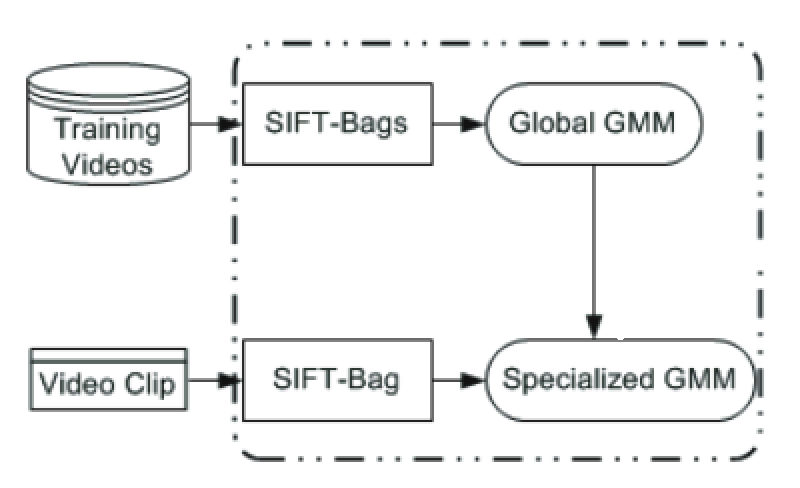
\includegraphics[scale=0.4]{./gmm.png}
	\caption{Illustration of building specialized GMMs for videos \cite{zhou2008sift}. The first step is to build a global GMM based on SIFT features of training data. The second step is to derive a specialized GMM from the global GMM for each video clip.}
	\end{figure}
	\paragraph{Global GMM built from training data} 
	Once all SIFT features of training data are loaded into memory, K-means clustering algorithm is applied on this bag of SIFT features to initialize $K$ centroids, where $K$ is a predefined number determining the number of Gaussian components of the global GMM. Afterward, the standard Expectation-Maximization (EM) is applied to obtain the global GMM. \\

	\noindent Suppose $X = \{x_1, \cdots, x_n\}$ are SIFT features extracted from training data, and $W = \{w_1, \cdots, w_K\}$ are the weights of respective Gaussian component. In E-step, the responsibilities of each SIFT feature to each Gaussian mixture component shall be computed. The below formula depicts the responsibility of $x_i$ to Gaussian component $k$.
	\begin{equation}
	Pr(k|x_i) = \frac{w_k \cdot \mathcal{N} (x_i ; \mu_k, \Sigma_k) }{\sum_{j=1}^{K}w_j \mathcal{N}(x_i ; \mu_j, \Sigma_j)}
	\end{equation}   

	\begin{equation}
	n_k = \sum_{i=1}^{n} Pr(k|x_i)
	\end{equation}

	\noindent In M-step, parameters of each Gaussian component are updated.
	\begin{equation}
	w_k = \frac{n_k}{n}
	\end{equation}

	\begin{equation}
	\mu_k = \sum_{j=1}^{n} \big( x_j \cdot \frac{Pr(k|x_j)}{n_k} \big)
	\end{equation}

	\begin{equation}
	\Sigma_k = \sum_{j=1}^{n} \big(  (x_j - \mu_k)(x_j - \mu_k)^T \cdot \frac{Pr(k|x_j)}{n_k} \big)
	\end{equation}

	\noindent The above E-step and M-step are repeated until convergence, and the resulting distribution of $X$ is modeled by Gaussian mixture models as 
	\begin{equation}
	p(x_i; \Theta) = \sum_{k=1}^{K} w_k \mathcal{N}(x_i; \mu_k, \Sigma_k)
	\end{equation}
	where $\Theta = \{w_1, \mu_1, \Sigma_1, \cdots \}$, $w_k$, $\mu_k$ and $\Sigma_k$ are the weight, mean and covariance matrix of the $k$th Gaussian component. 

	\paragraph{Specialized GMM by adaption}
	The specialized GMM for video clip is built on the global GMM. Given $Z = \{z_1,\cdots,z_H\}$ as the SIFT features extracted from one video clip that is being modeled, a modified EM algorithm is used to calculate the specialized parameters for this video clip. \\

	\noindent In E-step, the posterior probability is calculated as
	\begin{equation}
	Pr(k|z_i) = \frac{w_k \cdot \mathcal{N} (z_i ; \mu_k, \Sigma_k) }{\sum_{j=1}^{K}w_j \mathcal{N}(z_i ; \mu_j, \Sigma_j)}
	\end{equation}   

	\begin{equation}
	n_k = \sum_{i=1}^{H}Pr(k|z_i)
	\end{equation}

	\noindent In M-step, mean vectors are updated as
	\begin{equation}
	E_k(Z) = \frac{1}{n_k} \sum_{i=1}^{H} Pr(k|z_i) z_i
	\end{equation}
	\begin{equation}
	\hat\mu_k = \alpha_k E_k(z) + (1 - \alpha_k) \mu_k
	\end{equation}

	\noindent where $\alpha_k = \sfrac{n_k}{(n_k + r)}$, and $r$ is adjusted empirically depending on $H$, the total number of SIFT features for each video clip.\\

	\noindent The E-step and M-step are repeated until convergence. In the end, specialized GMM is modeled as $\hat\theta = \{\hat\mu_1, \cdots, \hat\mu_K \}$. It is worthy noting that all video clips are thus converted into equal size vectors if $\hat\theta$ is treated as a vector.

\subsection{Distance Calculations}
	Now that videos are represented in either stack of histograms or specialized GMM, it is time to calculate video-to-video distance for these two representations. For bag of word model, EMD is incorporated into distance calculation. Given the property that EMD only needs the best matches between segments, the distance between videos with different frames could also be calculated. This idea is originally proposed by Xu and Chang \cite{xu2007visual}, and it is now extended to Aligned Space-Time Pyramid Matching \cite{duan2012visual}. For specialized GMM representation, the author \cite{zhou2008sift} propose a distance formula generated from Kullback-Leibler divergence based on the assumption that the covariance matrices are unchanged during the Maximum a Posteriori adaption process.
	
	\subsubsection{Aligned space-time pyramid matching}
	Let's say there are two videos: $P = \{p_1, \cdots, p_m\}$ and video $Q = \{q_1, \cdots, q_n\}$, where $p_i$ and $q_i$ are the respective histograms in $P$ and $Q$. After attaching equal signatures to $P$ and $Q$ separately based on their number of histograms, $P$ and $Q$ are transformed into
	$$P = \{(p_1, 1 / m),...,(p_m, 1 / m) \}$$
	$$Q = \{(q_1, 1 / n),...,(q_n, 1 / n) \}$$
	
	\noindent Given the above representation, the distance between $P$ and $Q$ are defined as follows:
	\begin{equation}
	D_{PQ} = \frac{\sum_{i=1}^m \sum_{j=1}^n d_{ij} f_{ij}}{\sum_{i=1}^m\sum_{j=1}^n f_{ij}} 
	\end{equation}
	where $[d_{ij}]$ is the ground distance matrix, $d_{ij}$ calculates the distance between $p_i$ and $q_j$, and $[f_{ij}]$ is the optimal flow that can be obtained by solving the below linear programming problem:
	\begin{eqnarray}
	\text{minimize} & \sum_{i=1}^{m}\sum_{j=1}^{n}d_{ij}f_{ij} \nonumber \\
	\text{subjective to} & f_{ij} \geq 0 \quad \quad 1 \leq i \leq m,  1 \leq j \leq n \nonumber \\
	&\sum_{j=1}^n f_{ij} \leq 1 / m \quad 1 \leq i \leq m \nonumber \\
	&\sum_{i=1}^m f_{ij} \leq 1 / n \quad 1 \leq j \leq n\nonumber \\
	&\sum_{i=1}^{m} \sum_{j=1}^n f_{ij} = 1 
	\end{eqnarray}

	\noindent According to \cite{duan2012visual}, the distance calculated through the above process refers to Level-0 distance, and the reason is because a video is treated as a whole rather than several subclips. To utilize the power of pyramid, each video clip is divided into $8^l$ nonoverlapped space-time volumes over multiple levels, $l = 1,\cdots, L-1$, where the volume size is set to be $\sfrac{1}{2^l}$ of the original video in width, height and temporal dimension. Figure 11 below demonstrates how video is divided into 8 sub videos at level one. 

	\begin{figure}[!ht]
	\centering
		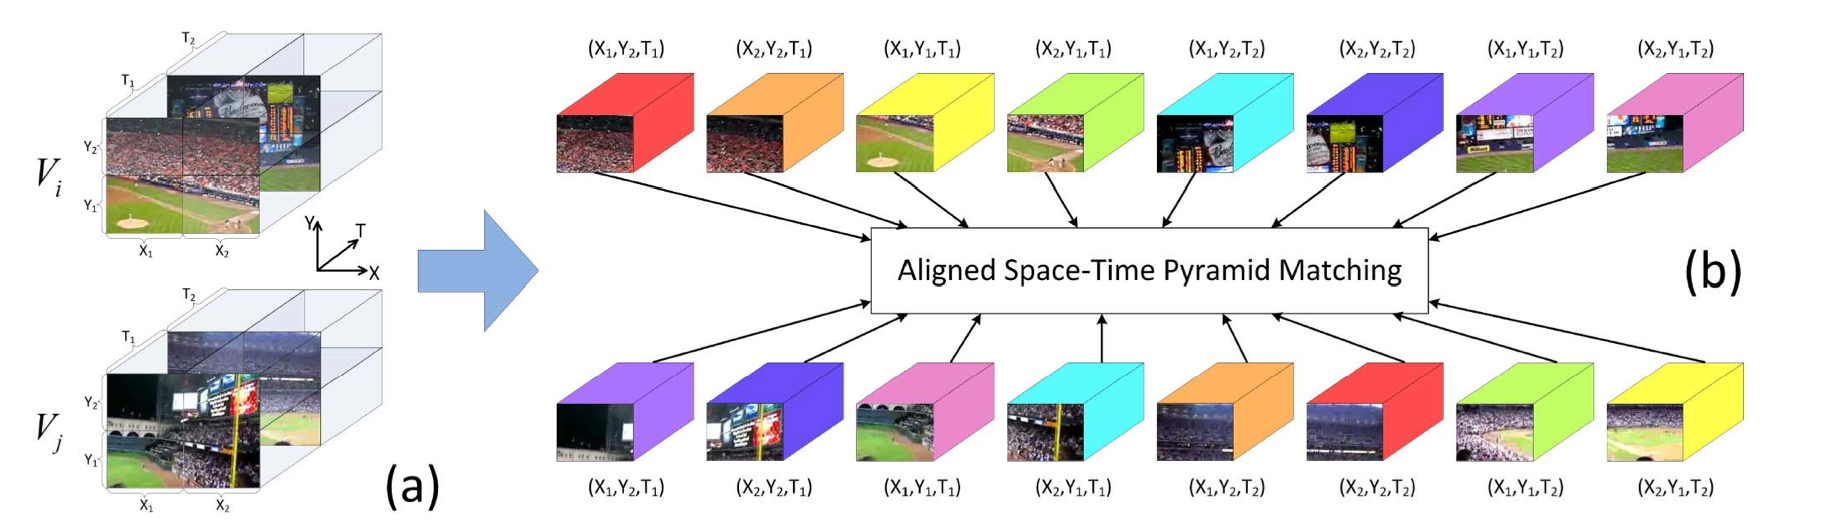
\includegraphics[width=1\linewidth]{./alignedST.png}
	\caption{Illustration of Aligned Space-Time Pyramid Matching at level one \cite{duan2012visual}. (a) Each video clip is divided into 8 sub videos. (b) Matched sub videos are painted in the same color.}
	\end{figure}

	\noindent Compared with level zero distance, the calculation of higher level distances require one more matching stage due to the increasing volumes in videos. Let's say 2 videos $P$ and $Q$ are divided into $8^l$ nonoverlapped space-time volumes at level $l$, and they are represented as
	$$P = (p_1, \cdots, p_R)$$
	$$Q = (q_1, \cdots, q_R)$$
	where $p_i$, $q_j$ are divided space-time volumes and $R$ equals to $8^l$. There are two matching stages to calculate distance between $P$ and $Q$ at level $l$. The first one is to calculate pairwise distance matrix $D$, where $D_{ij}$ is the EMD distance between $p_i$ and $q_j$. As a result, the shape of $D$ is $R^2$ because there are in total $R^2$ matches between space-time volumes of $P$ and $Q$. The additional stage is to align these pairwise distances. After solving the below linear programming problem using integer-flow EMD, those space-time volumes in $P$ and $Q$ are explicitly aligned. 
	\begin{eqnarray}
	& \hat F_{ij} = \argmin{F_{ij}} \sum_{i = 1}^{R} \sum_{j=1}^{R} F_{ij} D_{ij}
	\nonumber \\
	\text{subject to} & \sum_{i=1}^{R} F_{ij} = 1, \quad \forall j \nonumber\\
	&\sum_{j=1}^{R} F_{ij} = 1, \quad \forall i
	\end{eqnarray}

	\noindent Finally, the aligned distance $D_l(P,Q)$ between $P$ and $Q$ at level $l$ can be directly calculated as below
	\begin{equation}
	D_l(P,Q) = \frac{\sum_{i=1}^R \sum_{j=1}^R \hat F_{ij} D_{ij}}{\sum_{i=1}^R \sum_{j=1}^R F_{ij}}
	\end{equation}

	\subsubsection{Distances between specialized GMMs}
	Similar to previous section, let's say there are two video $P$ and $Q$. They are represented as two specialized GMM shown as below.
	$$P = (\mu_1^p, \cdots, \mu_K^p)$$
	$$Q = (\mu_1^q, \cdots, \mu_K^q)$$
	Given global GMM as $\Theta = \{w_1, \mu_1, \Sigma_1, \cdots\}$, the distance of $P$ and $Q$ is
	\begin{equation}
	d(P,Q) = \frac{1}{2} \sum_{k= 1}^{K} w_k (\mu_k^p - \mu_k^q)^T \Sigma_k^{-1} (\mu_k^p - \mu_k^q)
	\end{equation}

\noindent Once video-to-video distances using above approaches are calculated, they will be transformed into Gaussian, Laplacian, ISD and ID kernels for recognition using SVM. Due to the poor performance of KNN, there is no experiment using KNN to recognize videos. 

\subsection{Other Approach: Concept Attributes}
The approaches introduced above are under direct classification category, which model test videos in Bow or GMM and predict their labels directly. However, in real word, many events in videos could be really complex. For example, in the behavior of ``changing a vehicle tire'', events like ``person opening a car'', ``person using wrench'' and ``person holding something'' may be involved. However, Bow and GMM representations fall to catch these low-level events. To be able to better understand complex events, researchers have proposed to use concept attributes to describe images and videos \cite{liu2013video,natsev2010ibm, natarajan2011bbn}. \\

\noindent There are three stages to use concept attributes.
\begin{enumerate}
	\item{\bf Build concept detectors}\\
	Firstly, a concept space $\mathcal{C}^K$, where each dimension encodes the value of a semantic property, is defined. This space is spanned by $K$ concepts $\{C_1, \cdots, C_K\}$. Next, $K$ concept detectors are built based on training data. Each concept detector produces one score of respective concept to each input data sample. 
	\item{\bf Represent data in concept attributes}\\
	Given the above $K$ concept detectors, each data sample is input to these six detectors, and each detector produces one score. As a result, each data sample produces a vector $\{c_1,\cdots, c_k\}$, where $c_i$ is the output score of $i$th concept detector. 
	\item{\bf Recognize event classes using concept attribute representations}\\
	Now videos are transformed into vectors of concept attributes. Such representations are input into classification models like SVM for recognition.
\end{enumerate}

\noindent There are many variations and improvements on the above three stages. For instance, detectors for images could also be used in videos, given that a video consists of multiple frames. If an image is represented as a $K$-dimensional vector, then a video is represented by a $W \times K$ matrix, where each row represents a vector of an image, and there are in total $W$ images. For details, please refer to \cite{liu2013video}. \\

\noindent Last but not least, there are at least two advantages of using concept attributes. The first one is recognizing complex events, which has already been explained. Secondly, pre-trained detectors or even detectors shared by others could also be used to boost recognition performance. Given the fact that the cost of labelling training data is high, the second advantage provides lots of benefits by leveraging available resources. 
